\chapter{El problema inverso}%
\lhead{\thepage}
\rhead{\textit{El problema inverso}} \\
\vspace{0.01\textheight}
\label{sec:inverso}
%\pagebreak

En las secciones previas abordamos el problema directo de transporte 
de radiación en la materia mediante la ETR. En síntesis, el problema 
directo consta de, dados los parámetros ópticos $a(\x)$, $b(\x)$, la función  
de fase $\eta(\hth\cdot \hth')$, la velocidad de la luz en el medio participante 
$c$, las fuentes internas $s$ y las condiciones iniciales y de contorno, 
encontrar la solución $\ut$ a la ecuación~\eqref{eq:RTE}.

Para el problema inverso en tomografía óptica, alguno de los parámetros 
ópticos es desconocido, 
o conocido sólo parcialmente, y se dispone de mediciones experimentales 
de detectores colocados en el contorno del dominio que se quiere analizar. 
A partir de las mediciones experimentales de estos detectores, 
el objetivo es la reconstrucción de uno o más de los parámetros ópticos. 
En el caso de tomografía por fluorescencia y tomografía de bioluminiscencia, lo que se intenta reconstruir 
son las fuentes $s$ en la ec.~\eqref{eq:RTE}~\cite{Klose2005,Klose2009,Ren2010}, 
que vienen relacionadas a los coeficientes de absorción de los 
cromoforos y fluoroforos. 

En el contexto de esta tesis, nos limitaremos a la reconstrucción del 
coeficiente de absorción, $a(\x)$. La reconstrucción de dicho coeficiente 
encuentra aplicaciones en tomografía de fluorescencia, y en tomografía óptica. 
La reconstrucción de las propiedades de absorción en tomografía óptica 
 permite la identificación de tumores~\cite{Zhu2005,Zhu2010,Fujii2016b}, 
la obtención de imagenes funcionales del cerebro humano~\cite{Boas2001,bluestone2001,Arridge1999}, 
y la caracterización de diferentes constituyentes del tejido 
humano para la obtención de imágenes en medicina. En 
este trabajo nos enfocamos en la reconstrucción del coeficiente 
de absorción, pero los algorítmos y las estrategias propuestas 
pueden ser fácilmente generalizadas para la reconstrución 
de otros parámetros. 

Generalmente, para aplicaciones 
en diágnostico y monitoreo en el tratamiento de tumores, 
se asume cierta información previa 
para el coeficiente de dispersión, 
$b(\x)$, obtenida por técnicas de obtención 
de imagenes de alta resolución~\cite{Althobaiti2017,Guven2003} \eg Resonancia Magnética. 
Este conocimiento previo obtenido por otras técnicas, también brinda 
información límitada en el parámetro óptico de absorción $a(\x)$, 
como pueden ser los coeficientes de absorción para ciertos tejidos óseos, 
o el aire en regiones como la traquea del cuello humano, como también 
se conocen cotas superiores e inferiores para dicho parámetro, 
lo que permite restringir el espacio de funciones donde se busca minimizar 
la función objetivo. El uso de técnicas de alta resolución, como la Resonancia 
Magnética, posee ciertas límitaciones, como el alto costo, la baja disponibilidad 
de este tipo de aparatos 
(lo que impone una dificultad a la hora de seguir la evolución de un tratamiento 
asistida por diagnóstico de imágenes), y adicionalmente los dispositivos 
utilizados en tomografía óptica son portables, lo que permite tenerlos disponibles 
para su uso en diversas situaciones. En la figura~\ref{fig:esquemainv} esquematizamos los problemas directos e inverso, tal como son 
tratados en esta tésis. 


\begin{figure}[h!]
\centering
  \includegraphics[width=\linewidth]{figuras/inv.pdf}\\
  \caption{
Grafico esquematico de los problemas directo e inverso, tal como son considerados 
en esta tésis.}
 \label{fig:esquemainv}
\end{figure}
Para la resolución del problema inverso, utilizamos el esquema \textit{MOBIR}, 
presentado en la sección siguiente. 

\section{El esquma \textit{MOBIR}}

\begin{wrapfigure}{l}{0.48\textwidth}
  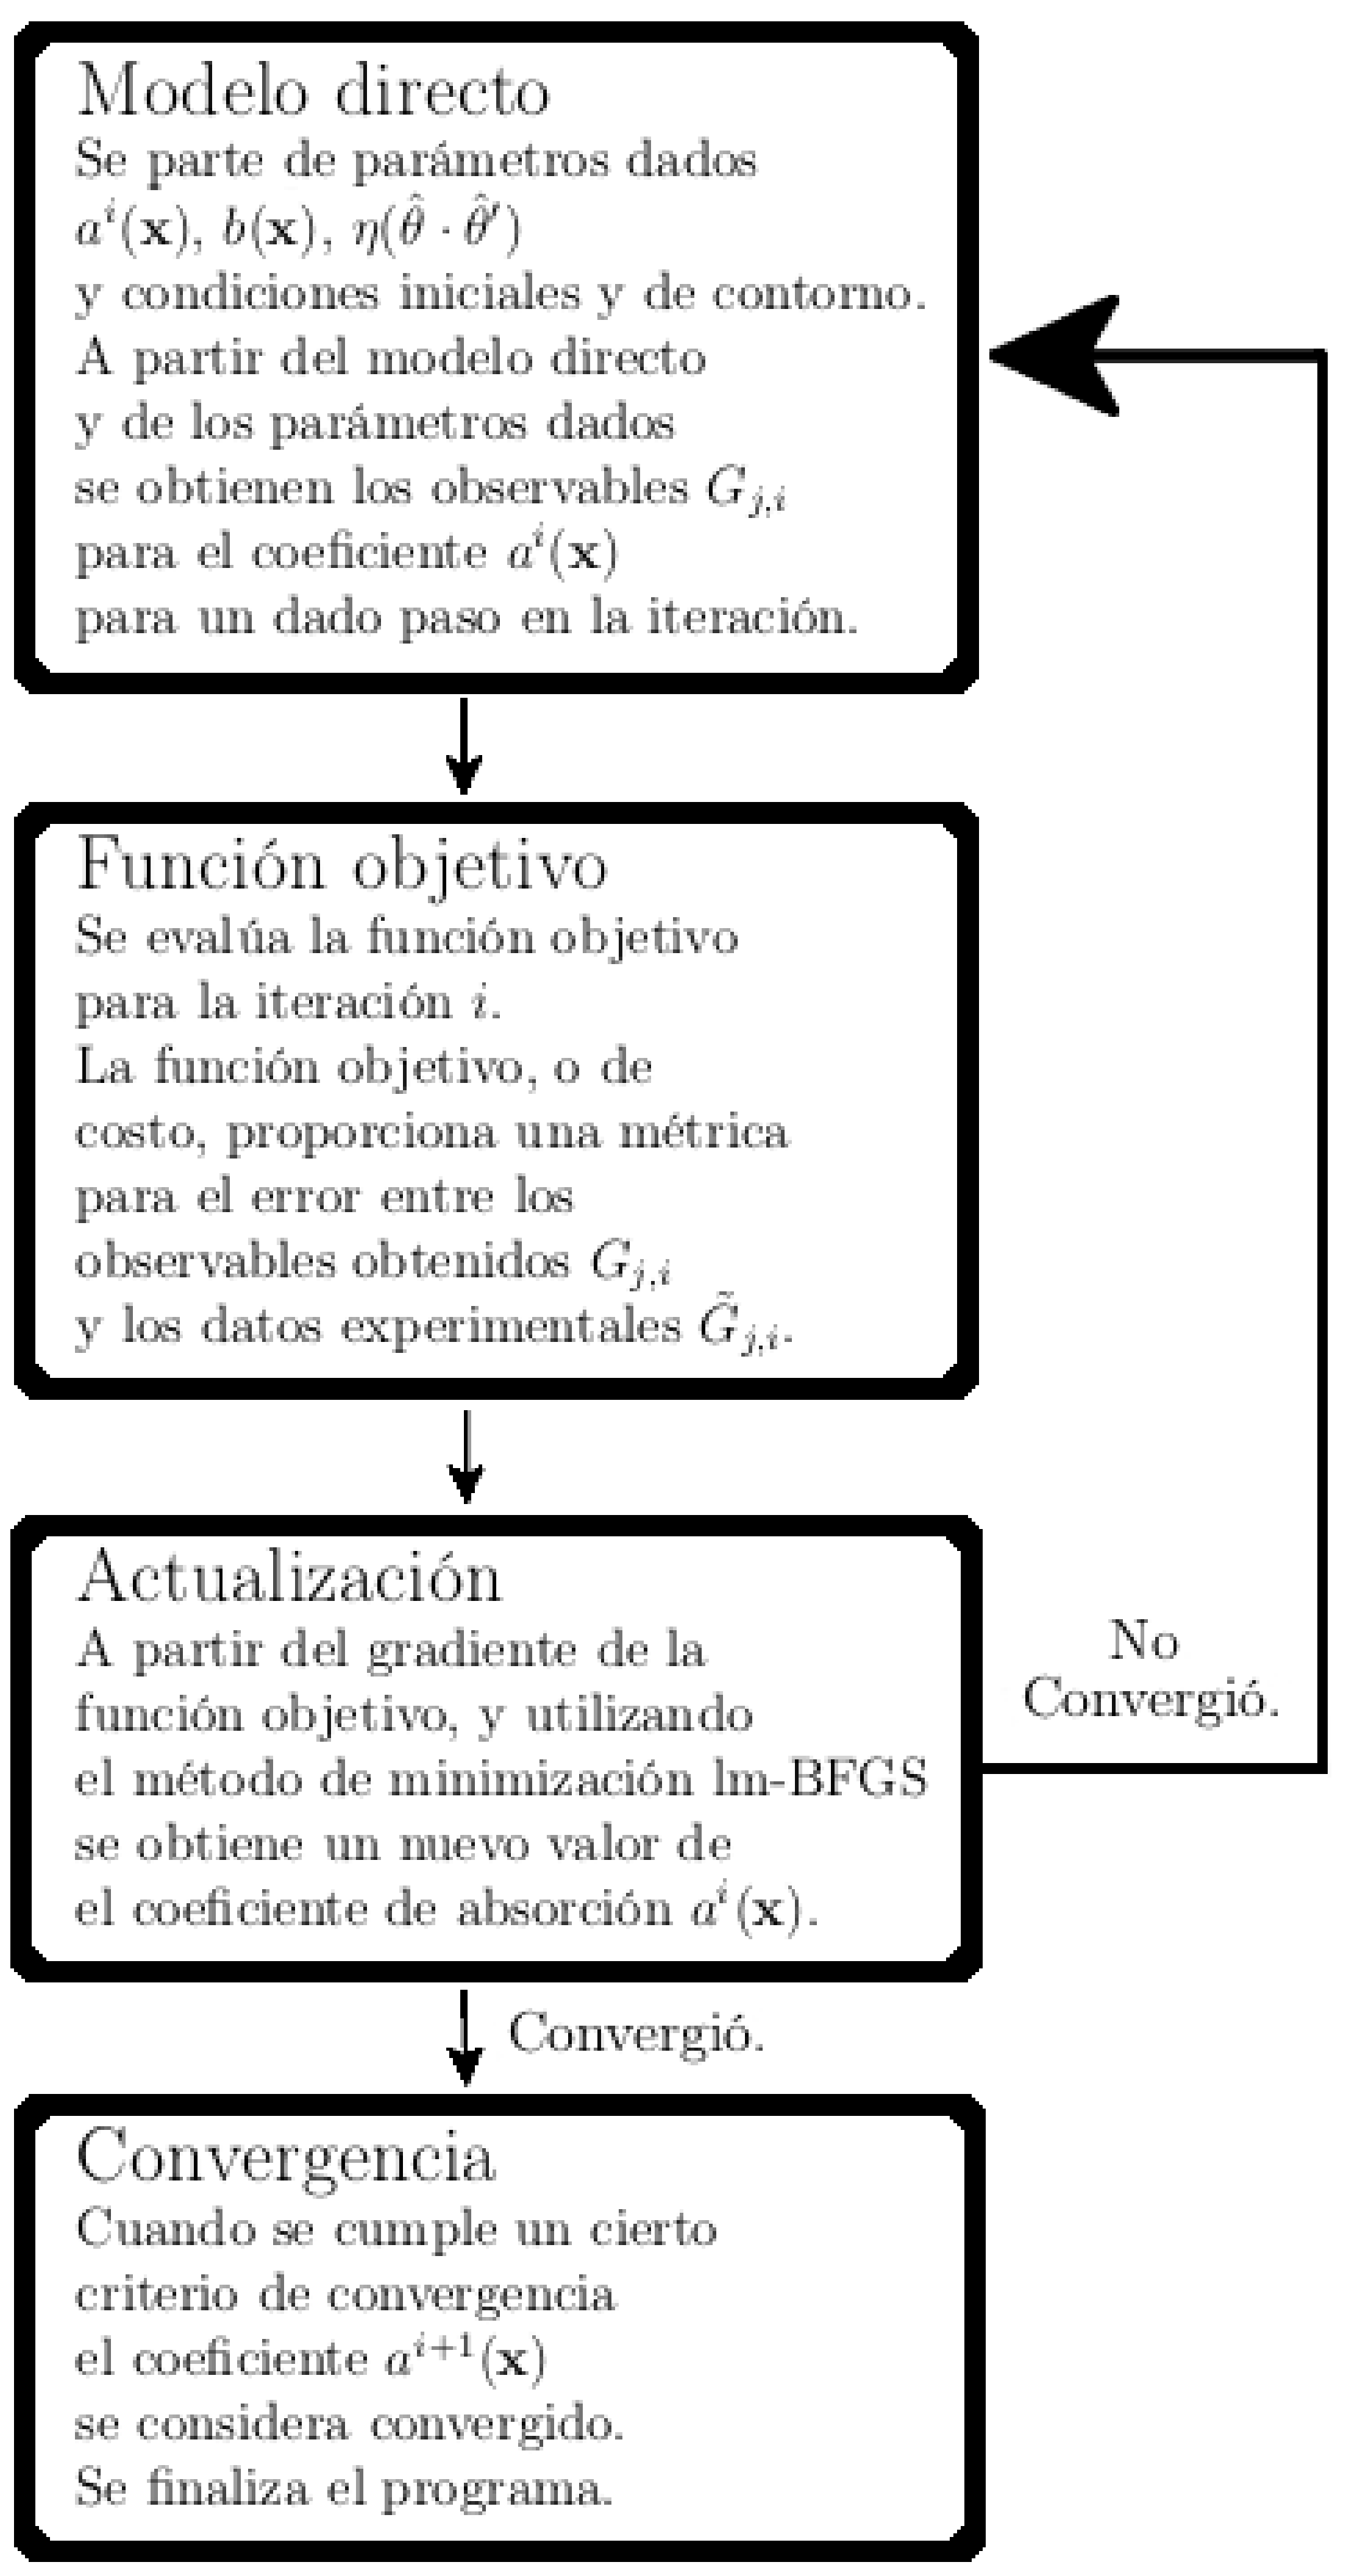
\includegraphics[width=0.48\textwidth]{figuras/mobir.eps}\\
  \caption{Esquema  MOBIR. El modelo directo es utilizado para obtener los observables simulados. Se evalúa el error entre los datos experimentales y los simulados por medio de la función objetivo. 
  Luego, utilizando un método de minimización, se actualiza el coeficiente $a(\x)^{i+1}$ a 
  ser utilizado en la iteración subsiguiente, hasta cumplir 
  un cierto criterio de convergencia. }
 \label{fig:mobir}
\end{wrapfigure}

En este tesis desarrollamos un algoritmo tipo MOBIR~\cite{Hielscher1999,Kim2010} (del inglés, {\em Model Based Iterative Image  
Reconstruction}). Este tipo de esquemas se basan en un modelo físico, y un método de minimización 
iterativo para la reconstrucción del parámetro deseado en el problema inverso.

El modelo físico utilizado es la Ecuación de Transporte Radiativo~\eqref{eq:RTE}. 
Para la minimización del funcional objetivo (que será introducido en una sección posterior) emplearemos el método de minimización 
de Broyden–Fletcher–Goldfarb–Shanno (BFGS) con uso de memoria reducido 
(lm-BFGS, de su sigla en inglés)~\cite{Byrd1995}. 

El problema inverso en tomografía óptica es resuelto como un problema de optimización 
no lineal. A partir de un valor inicial para el coeficiente de absorción $a(\x)^0$, 
el coeficiente de absorción es buscado de forma iterativa, actualizando su valor 
en cada iteración mediante el método lm-BFGS, el cual es un caso particular 
de los métodos de cuasi-Newton~\cite{Nocedal2006,Klose2003QN,Ren2006}. 
Partiendo del valor inicial $a(\x)^0$, el cual en general es estimado 
a partir de información obtenida de manera previa por otros métodos de imagenes, 
el coeficiente de absorción es 
\clearpage
\noindent actualizado en cada paso de la iteración $i+1$, según~\cite{Klose2003QN}
\begin{equation}
\mathbf{a}(\x)^{i+1}=\mathbf{a}(\x)^{i}+\alpha^i  \mathbf{d}^i
\label{eq:update}
\end{equation}
donde $\mathbf{a}(\x)^{i}$ debe ser interpretado como el 
vector obtenido a partir de el coeficiente de absorción en el 
dominio espacial $\Omega$  
discretizado, con $\alpha^i$ el largo del paso de Newton, y $\mathbf{d}^i$ 
la dirección de descenso. En el caso del método de Newton (o de descenso más rápido), la dirección de 
descenso vendrá dada por el gradiente $-\nabla_a g $ de la función objetivo $g[u]$ (a ser definida en secciones posteriores). 
En el contexto de esta tesis emplearemos el método lm-BFGS, ya que este método a 
mostrado ser eficiente en el contexto de tomografía óptica~\cite{Klose2003QN,Ren2006,
Prieto2017}. 




\subsection{El operador de transporte}

\subsection{Cálculo del gradiente de la función objetivo mediánte el formalismo 
del operador adjunto}
\section{Reconstrucciones numéricas}
\label{sec:inverseres}
\section{Consecuencias de la capa límite}
